\documentclass[border=8pt]{standalone}
\usepackage{pgfplots}
\pgfplotsset{compat=1.18}
\begin{document}
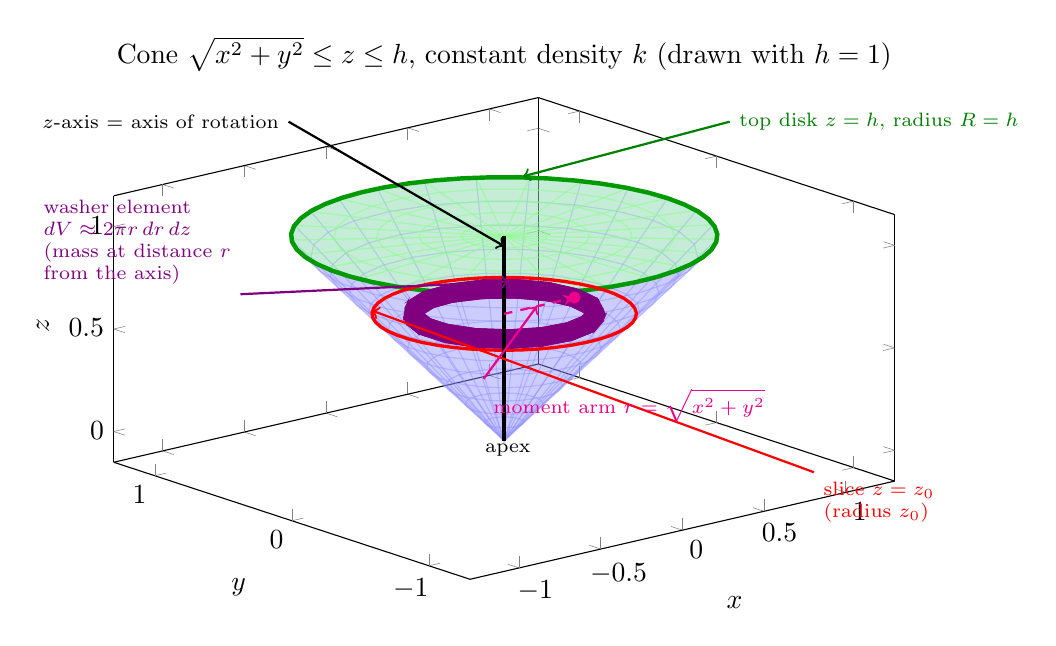
\begin{tikzpicture}
\begin{axis}[
  width=11.5cm, height=10cm,
  view={-40}{16},
  xlabel={$x$}, ylabel={$y$}, zlabel={$z$},
  xmin=-1,xmax=1, ymin=-1,ymax=1, zmin=0,zmax=1,
  ztick={0,0.5,1},
  axis equal image,
  enlargelimits=0.15, clip=false,
  title={Cone $\sqrt{x^2+y^2}\le z\le h$, constant density $k$ (drawn with $h=1$)},
  every title/.style={font=\small}]

  \addplot3[surf, color=blue!45, opacity=0.25, shader=flat,
            domain=0:1, domain y=0:360, samples=12, samples y=26]
    ({x*cos(y)},{x*sin(y)},{x});

  \addplot3[surf, color=green!45, opacity=0.35, shader=flat,
            domain=0:1, domain y=0:360, samples=6, samples y=26]
    ({x*cos(y)},{x*sin(y)},{1});

  \addplot3[green!60!black, ultra thick, domain=0:360, samples=48]
    ({cos(x)},{sin(x)},{1});

  \addplot3[red, very thick, domain=0:360, samples=48]
    ({0.62*cos(x)},{0.62*sin(x)},{0.62});

  \addplot3[surf, color=violet, opacity=0.95, shader=flat,
            domain=0:360, domain y=0:360, samples=18, samples y=9]
    ({(0.43+0.045*cos(y))*cos(x)},{(0.43+0.045*cos(y))*sin(x)},{0.62+0.045*sin(y)});

  \addplot3[black, ultra thick] coordinates {(0,0,0) (0,0,1)};
  \addplot3[magenta, thick, dashed, -stealth] coordinates {(0,0,0.62) (0.43,0,0.62)};
  \addplot3[magenta, only marks, mark=*] coordinates {(0.43,0,0.62)};

  \node[font=\scriptsize,violet,align=left] (Lv) at (axis description cs:0.03,0.70)
      {washer element\\ $dV\approx 2\pi r\,dr\,dz$\\ (mass at distance $r$\\ from the axis)};
  \draw[violet,thick,->] (Lv.south east) -- (axis cs:0.28,0.30,0.66);

  \node[font=\scriptsize,red,align=left] (Lr) at (axis description cs:0.98,0.16)
      {slice $z=z_0$\\ (radius $z_0$)};
  \draw[red,thick,->] (Lr.north west) -- (axis cs:-0.44,0.44,0.62);

  \node[font=\scriptsize,green!50!black] (Lg) at (axis description cs:0.98,0.95)
      {top disk $z=h$, radius $R=h$};
  \draw[green!50!black,thick,->] (Lg.west) -- (axis cs:0.72,0.72,1.0);

  \node[font=\scriptsize] (Lz) at (axis description cs:0.06,0.95)
      {$z$-axis = axis of rotation};
  \draw[black,thick,->] (Lz.east) -- (axis cs:0,0,0.95);

  \node[font=\scriptsize,magenta] (Lm) at (axis description cs:0.66,0.36)
      {moment arm $r=\sqrt{x^2+y^2}$};
  \draw[magenta,thick,->] (Lm.north west) -- (axis cs:0.20,0.0,0.62);

  \node[font=\scriptsize] at (axis cs:0.14,0.14,-0.10) {apex};
\end{axis}
\end{tikzpicture}
\end{document}
